\section{Working hours}

This attack aims to extract information about the working hour behaviour of a target.
This should be achieved by displaying the pattern of the target in form of a weighted scatter plot sorted by hour per weekday and by comparing those patterns between several targets.
There are several possible vectors for this attack:

\begin{itemize}
    \item Information about the sleep rhythm of the target.
    \item Detect whether the target is a person working regular shifts from from Monday to Friday or rather an open-source contributor working in their leisure time.
    \item Detect anomalies such as automated programs, which contribute to a project on a regular basis.
    \item Compare the working hour patterns of several people in the same project or organization. This could, for instance, be used to infer relationships between colleagues, based on an equal working shifts.
\end{itemize}

Additionally a clustering will be performed to find anomalies, common patterns and to evaluate the results of this analysis.
As we are only interested in contributors with a representative amount of commits, all contributors with less than one hundred commits in the last year have been excluded.
This reduced the amount of considered contributors from 175.000 to about 10.300.


\subsection{Implementation}\label{punchcard-implementation}

The initial data for this analysis are the commit timestamps of the target.
These commit timestamps are then converted into a different format, which represents the occurrences of commit per hour per weekday over the last year.
The result is a simple vector with length 168, which corresponds seven days with 24 hours each.
I will refer to this representation hereafter as a \emph{punchcard}.

\begin{minted}{python}
def preprocess(commits):
    punchcard = [0] * 168
    for commit in commits:
        hour = commit.commit_time.hour # returns 0-23
        weekday = = commit.commit_time.weekday() # returns 0-6

        index = weekday*24 + hour
        punchcard[index] += 1

\end{minted}
\begingroup
\captionof{listing}{Data preprocessing}\label{lst:puchcard-preprocessing}
\endgroup

The data transformation is achieved by incrementing the field of the respective weekday and hour by one for each commit, as can be seen in~\ref{lst:puchcard-preprocessing}.
The resulting punchcard vector is then stored in the database for faster and easier analysis in the next steps.

\begin{figure}[H]
    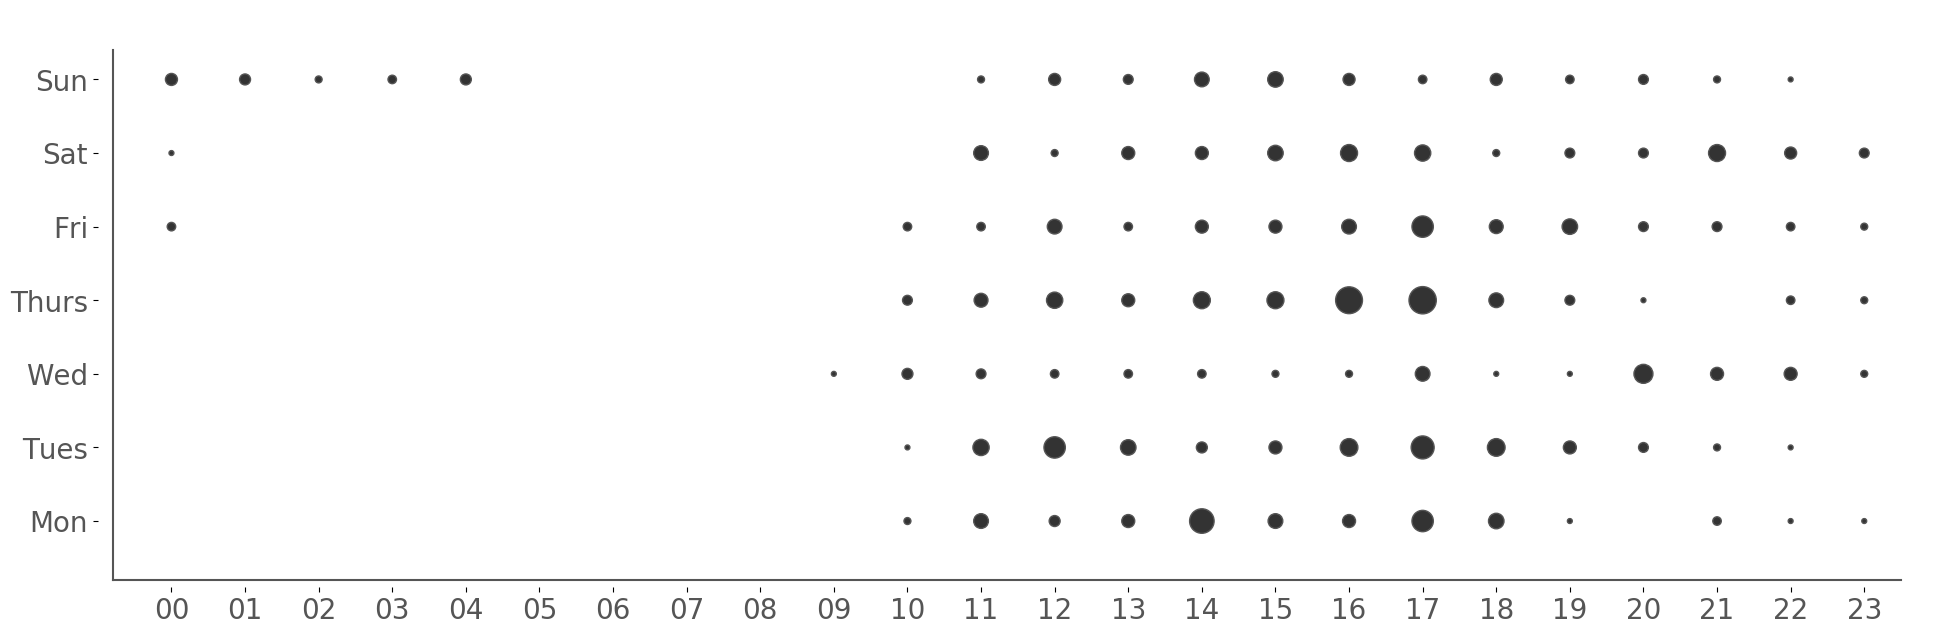
\includegraphics[scale=0.32]{./graphs/analysis/ordered-punchcard}
    \centering
    \caption{Punchcard of the author.}\label{fig:working-hour-rhythm-author}
\end{figure}



\subsection{Punchcard Clustering}

To find common work patterns, several cluster cluster algorithms have been performed on the aggregated data.
The Python \emph{scikit} framework has been used for this purpose, as it features nine different clustering methods and provides good documentation and abstraction from the underlying clustering logic~\footnote{`Clustering' scikit-learn.org, http://scikit-learn.org/stable/modules/clustering.html (accessed, 24.04.2018)}.
For the task of finding similar punchcard patterns in the data, a clustering algorithm is required, which can operate on a high-dimensional dataset with an unknown amount of clusters
Scikit provides three different clustering algorithms, which can handle an unknown amount of clusters.

\subsubsection{Mean-Shift}

\begin{figure}[H]
    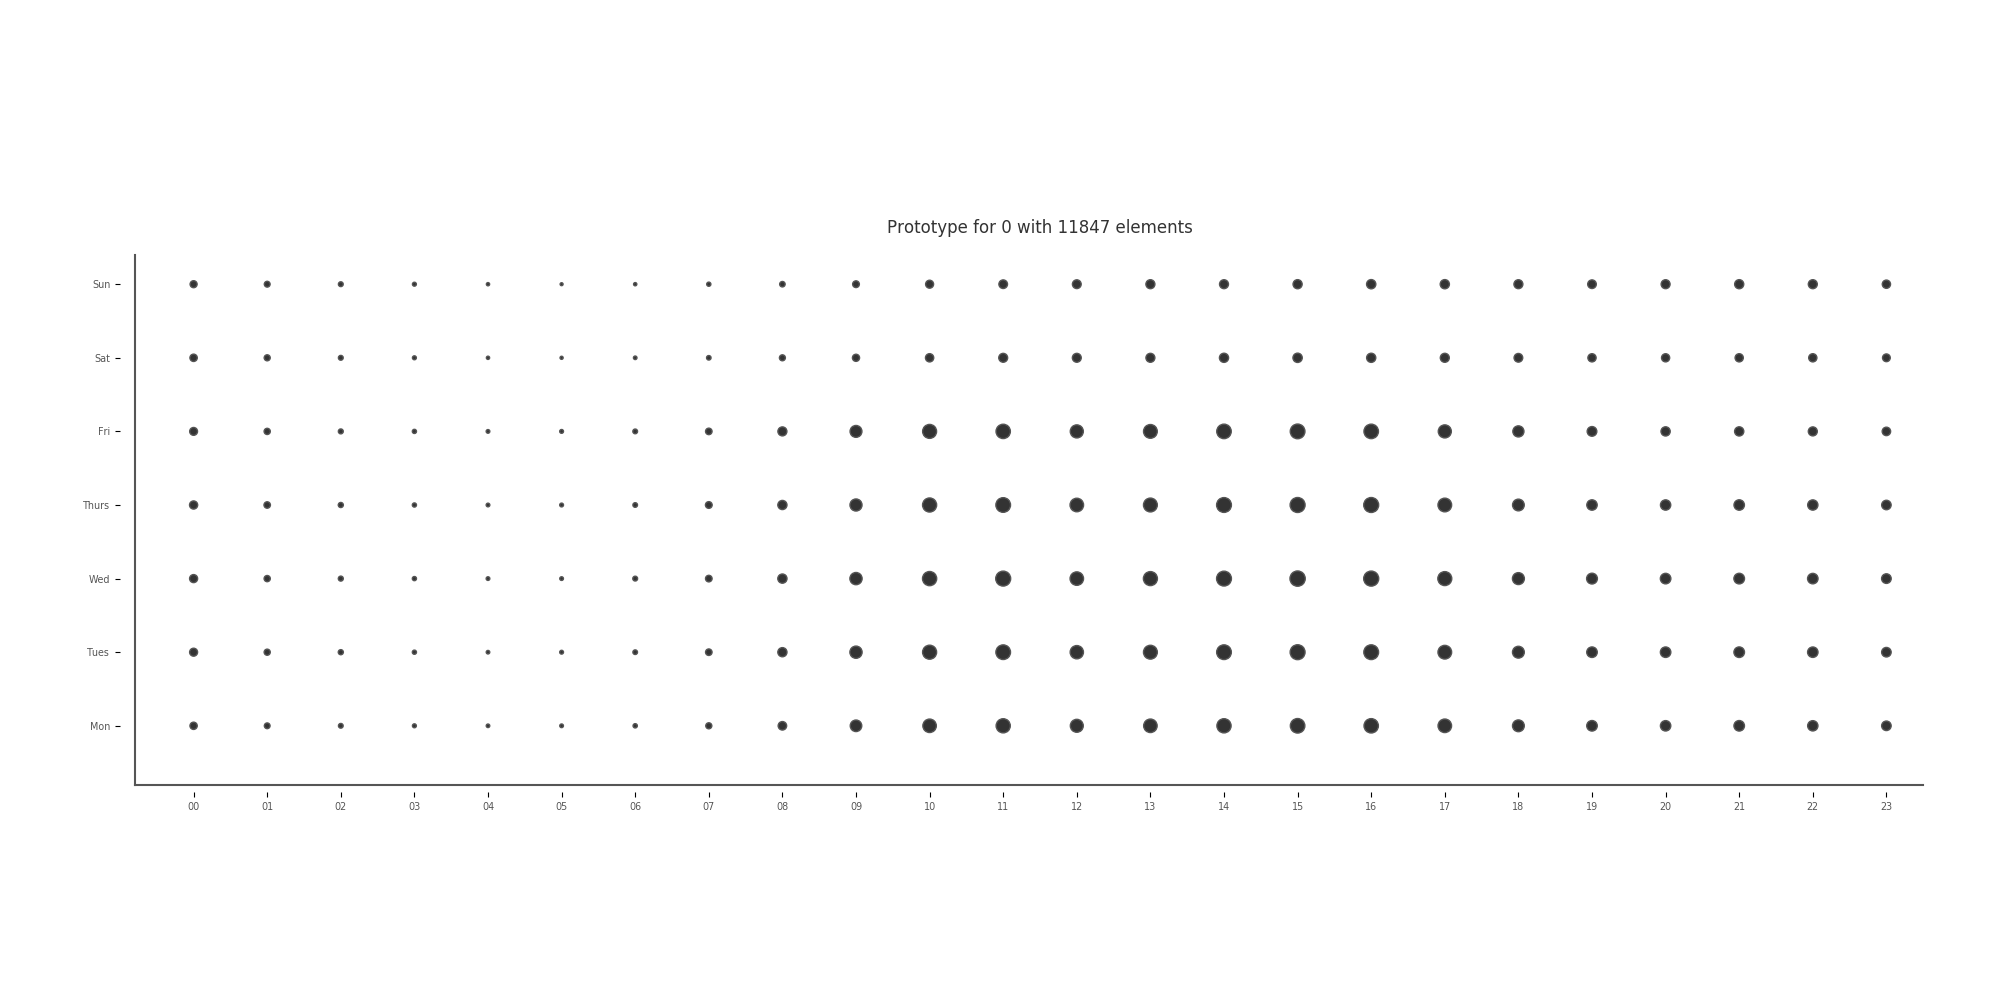
\includegraphics[scale=0.32]{./graphs/analysis/supercluster}
    \centering
    \caption{Supercluster found by mean-shift clustering.}\label{fig:working-hour-rhythm-author}
\end{figure}


\subsubsection{DBSCAN}

\subsubsection{Affinity Propagation}
Affinity Propagation considers similarities between all data points to find clusters.
The memory requirements for this method scale quadratically for non-sparse sets with the number of the data points~\cite[p.~ii]{article:Frey972}
About 13 \ac{gb} memory have already been used with a sample of roughly 10.000 data points and becomes thereby impractical for larger scale analyses.
This clustering algorithm features a promising approach, as it utilizes a method similar to message passing, to find an \emph{exemplar}, which resembles the representative of a cluster, and its surrounding cluster member.
However it has to be noted, that this clustering method is sometimes a little too detailed, as it, for instance, split very similar patterns into two or more different clusters.


